\setcounter{figure}{0} 
\setcounter{table}{0}
\setcounter{footnote}{0}
\setcounter{equation}{0}
\pagestyle{fancy}
\fancyhf{}
\renewcommand{\chaptermark}[1]{\markboth{\MakeUppercase{#1 }}{}}
\renewcommand{\sectionmark}[1]{\markright{\thesection~ #1}}
\fancyhead[RO]{\bfseries\rightmark}
\fancyhead[LE]{\bfseries\leftmark}
\fancyfoot[RO]{\thepage}
\fancyfoot[LE]{\thepage}
\renewcommand{\headrulewidth}{0.5pt}
\renewcommand{\footrulewidth}{0pt}

\makeatletter
\renewcommand\thefigure{A.\arabic{figure}}
\renewcommand\thetable{A.\arabic{table}} 
\makeatother

\chapter{Annexe}
\graphicspath{{Annexe1/figures/}}
%==========================================================================

%    Annexe

%===========================================================================


\section{Annexe A}
Dans cet annexe, nous pr�sentons les interfaces de SlipStream qui affichent toutes les informations sur les VMs de la solution Big Data apr�s le lancement du d�ploiement.\\

La figure \ref{fig:fig1} pr�sente la vue globale du d�ploiement en �tat 'Ready'.
\begin{figure}[H]\centering
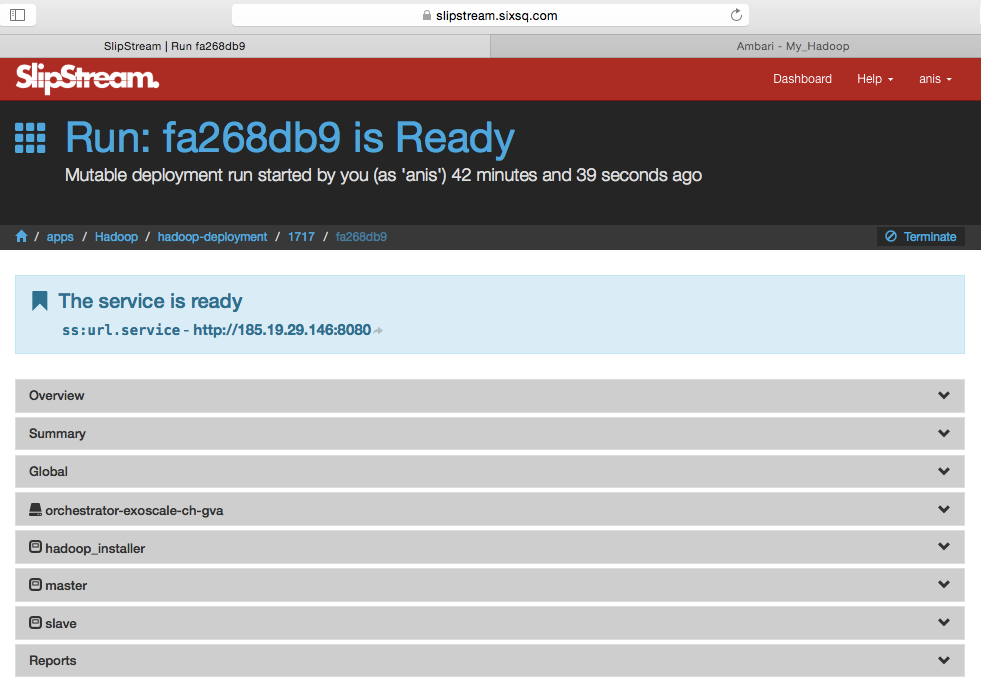
\includegraphics[scale=0.64]{1-overview.png}
\caption{Vue globale d'un d�ploiement de Hadoop}
\label{fig:fig1}
\end{figure}

\newpage
La figure  \ref{fig:fig2} illustre la section de la VM 'hadoop installer'.
\begin{figure}[H]\centering
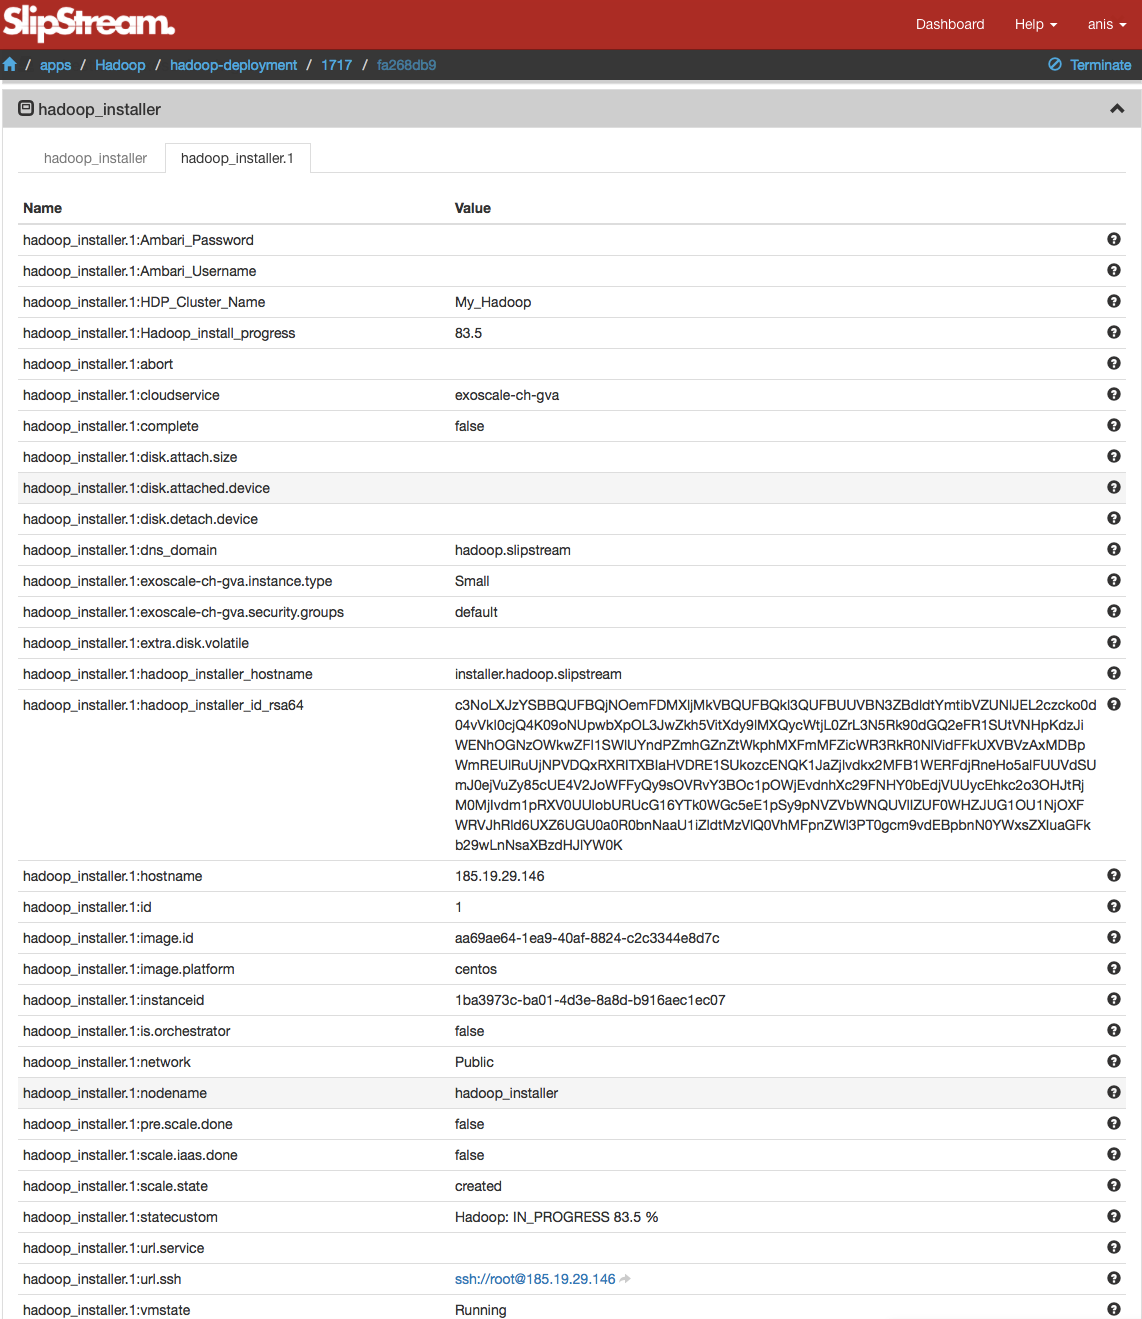
\includegraphics[scale=0.565]{2-hadoop-installer.png}
\caption{Informations sur la VM 'hadoop installer'}
\label{fig:fig2}
\end{figure}

La figure \ref{fig:fig3}  pr�sente la section de la VM 'master'.\\
\begin{figure}[H]\centering
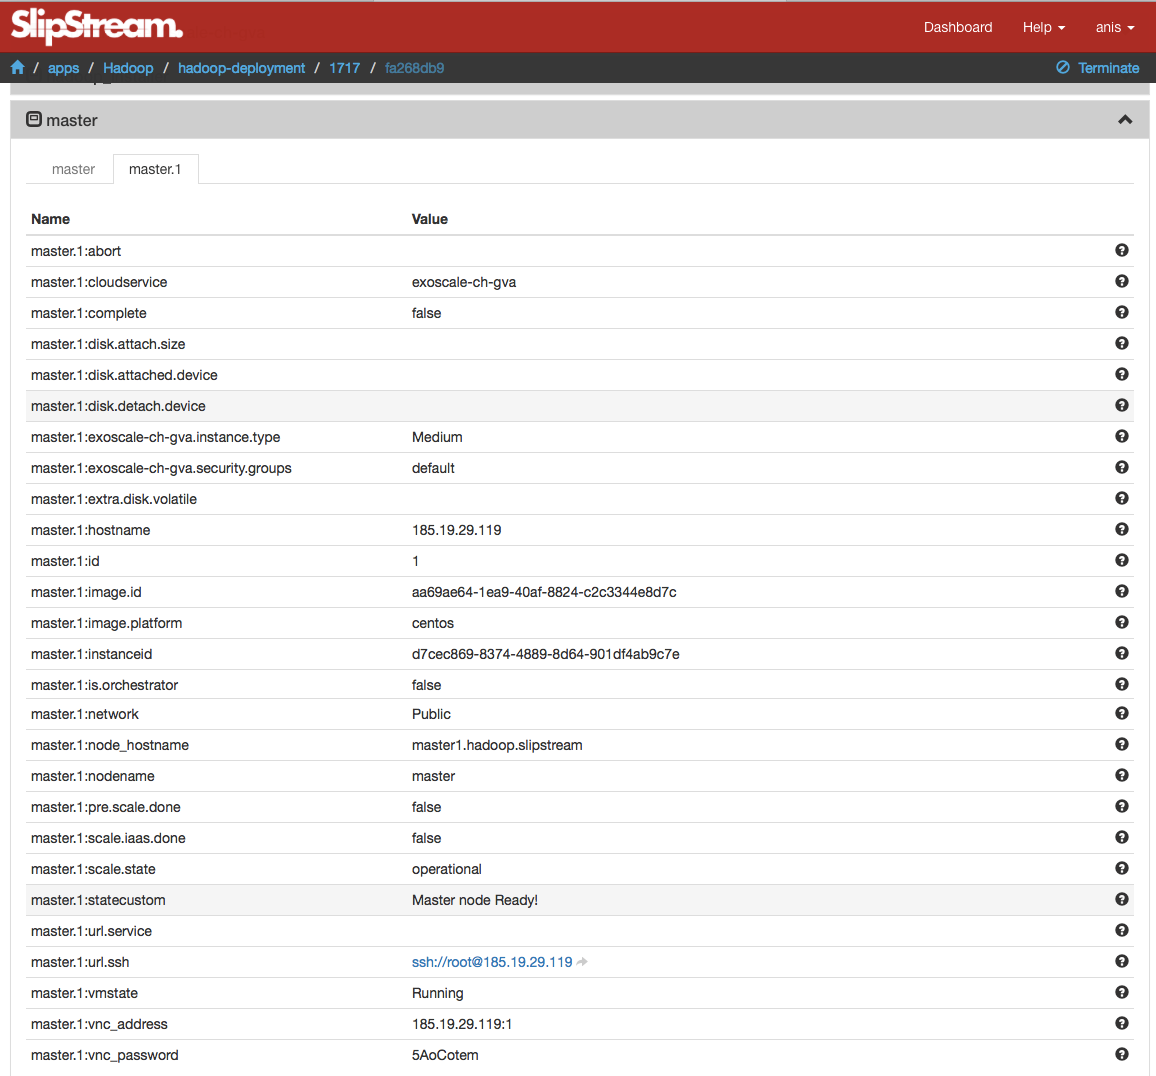
\includegraphics[scale=0.56]{3-master.png}
\caption{Informations sur la VM 'master'}
\label{fig:fig3}
\end{figure}

\newpage
La figure \ref{fig:fig4} pr�sente la section de toutes les VM slave du cluster.\\
\begin{figure}[H]\centering
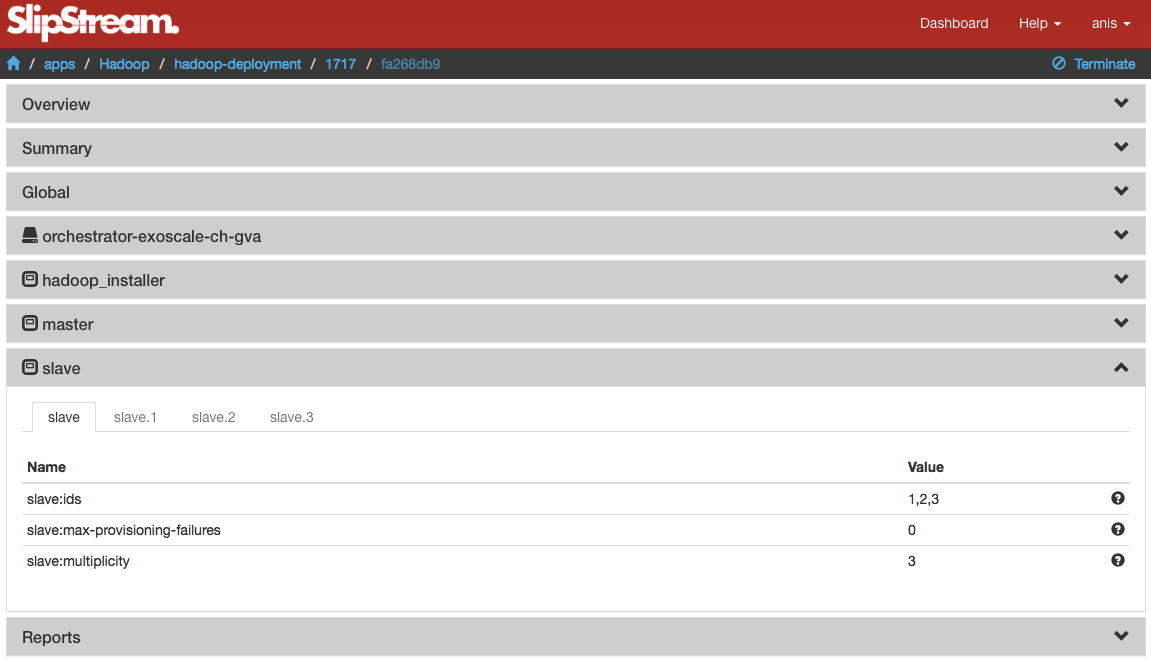
\includegraphics[scale=0.57]{4-slave.png}
\caption{Information sur les VMs slaves du cluster}
\label{fig:fig4}
\end{figure}


\newpage
Une fois le d�ploiement termin�, SlipStream envoie � ses utilisateurs tous les Logs du d�ploiement afin de les t�l�charger. La figure  \ref{fig:fig5}  pr�sente les Logs de notre d�ploiement de Hadoop.\\
\begin{figure}[H]\centering
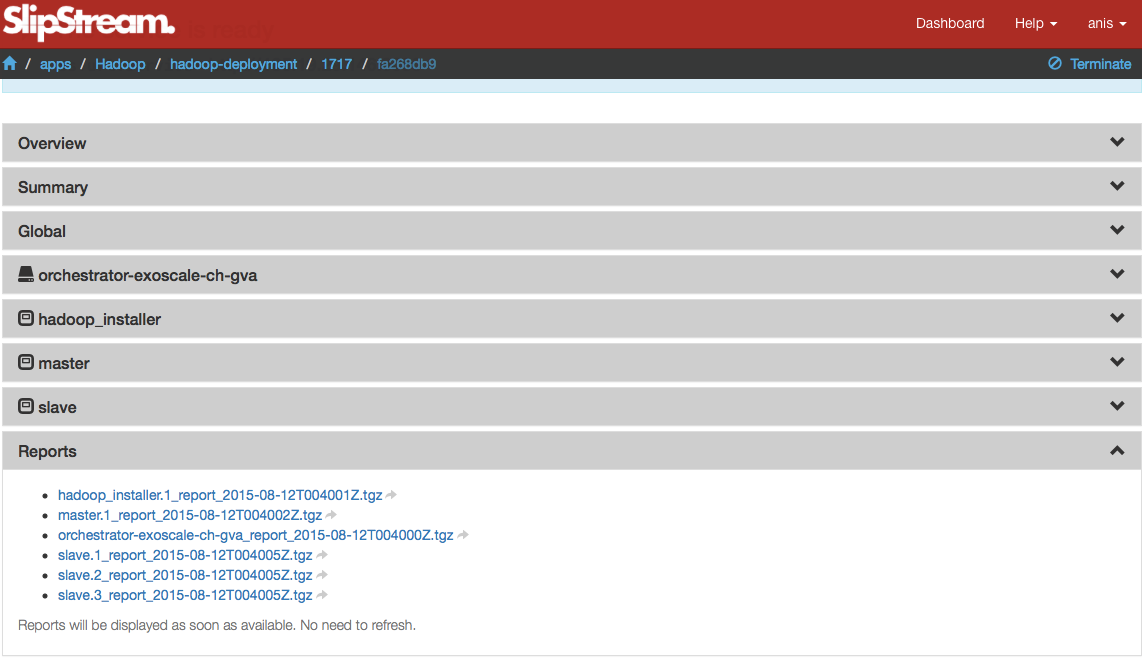
\includegraphics[scale=0.57]{5-log.png}
\caption{Logs du d�ploiement de Hadoop}
\label{fig:fig5}
\end{figure}





\newpage

\section{Annexe B}
Dans l'annexe B, nous pr�sentons les services de Hadoop que nous pouvons ajout� au cluster tout en utilisant 'Ambari server' d�ploy� dans la VM 'hadoop installer'.\\

La figure  \ref{fig:fig6}  illustre la section � Services � de l'interface d'administration.
\begin{figure}[H]\centering
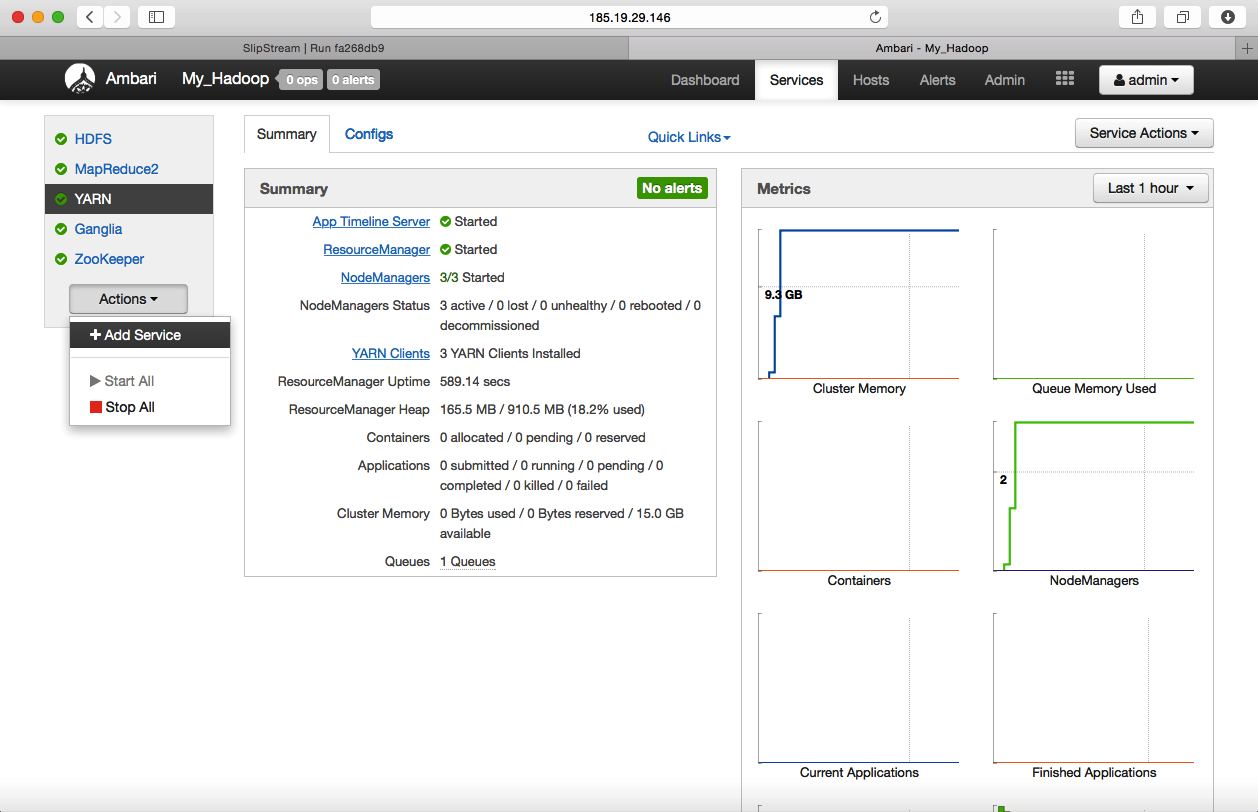
\includegraphics[scale=0.5]{6-ambari.png}
\caption{Section services de l'interface d'administration Ambari}
\label{fig:fig6}
\end{figure}


\newpage
La figure  \ref{fig:fig7} pr�sente tous les services que nous pouvons ajouter � notre cluster d�ploy�.

\begin{figure}[H]\centering
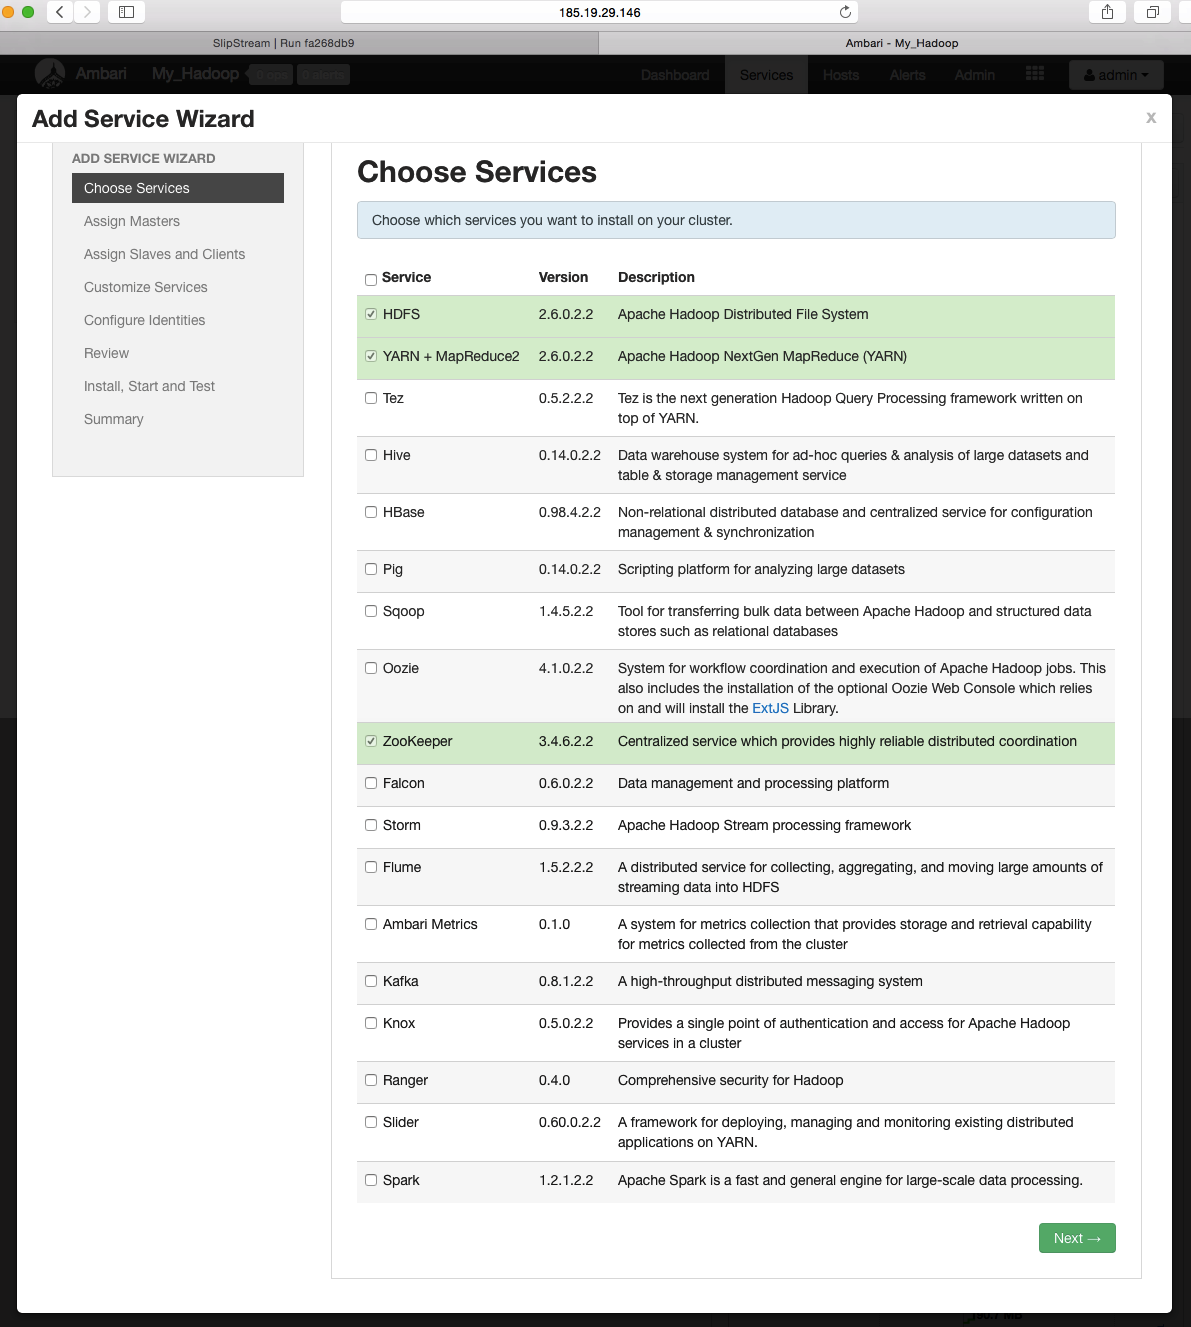
\includegraphics[scale=0.55]{7-services.png}
\caption{Interface d'Ambari pour ajouter les services de Hadoop}
\label{fig:fig7}
\end{figure}




\newpage

\section{Annexe C}
Dans cet annexe, nous d�taillons la configuration des ports pour notre solution. Le tableau Tab \ref{tab:ports} pr�cise les ports par d�faut qui doivent �tre ouverts pour permettre � tous les composants de communiquer les uns avec les autres.\\


\begin{table}[ht]
	\centering
	\caption{Ports utilis�s par notre solution Big Data}
	\footnotesize
	\begin{tabularx}{\linewidth}{|>{\bfseries \vspace*{\fill}}X ||>{\centering{}\vspace*{\fill}}X|>{\vspace*{\fill}}X<{\centering{}}|}	
			\hline 
			Service/composant & \bfseries Ports par d�faut & \bfseries Protocole \\
			\hline \hline
			HDFS : NameNode WebUI		&	50070/50470	&	TCP (Transmission Control Protocol)	\\
			\hline
			HDFS : NameNode metadata service		&	8020/9000	&	TCP	\\
			\hline
			HDFS : DataNode		&	50075/50475/50010/ 0.0.0.0:8010	&	TCP	\\
			\hline
			HDFS : Secondary NameNode		&	50090	&	TCP	\\
			\hline
			MapReduce : History Server WebU		&	19888	&	TCP	\\
			\hline
			YARN : Resource Manager		&	8025 	&	TCP	\\
			\hline
			YARN :RM Admin		&	8141 	&	TCP	\\
			\hline
			YARN : Container Manager		&	0.0.0.0:45454	&	TCP	\\
			\hline
			YARN : Applications Manager		&	8050 	&	TCP	\\
			\hline
			ZooKeeper Server		&	2888/3888/2181	&	TCP	\\
			\hline
			Ganglia Server		&	8660/8651/61/62/63	&	TCP	\\
			\hline
			Ganglia Monitor		&	8660	 &	TCP	\\
			\hline
			Ambari Server		&	8080/8440/8441	&	TCP	\\
			\hline
			Nagios Server		&	80	&	TCP	\\
			\hline
			Connexion SSH		&	22	&	TCP	\\
			\hline
			VNC Server		&	5900 	&	TCP	\\
			\hline
			Connexion master-slaves		&	40000..61000	&	TCP	\\
			\hline
			Dnsmasq		&	53	&	UDP (User Datagram Protocol)	\\
			\hline			
	\end{tabularx}
	\label{tab:ports}
\end{table}